\section*{Durchführung}
Wie bereits erläutert weißt das SIR-Modell einige Schwächen auf unter Anderem wird in dem Modell davon ausgegangen dass jeder Mensch im Schnitt acht Kontakte, je nach Modellierung, zu anderen Menschen hat. In unserem Programm wird dies dynamisch geregelt, dort gibt es einen Raster welcher einem Schachbrett ähnelt auf diesem beliebig großem rechteckigem \glqq{}Raster\grqq{} lassen sich an jeder $ x,y $ Position Zellen positionieren. So kann es Zellen geben welche sehr viele Nachbarn haben aber auch Zellen welche gar keinen Nachbar haben. Einen exemplarischen Raster sieht man in  Abbildung \ref{fig:Raster}. Auf diesem 3x3 Raster befinden sich aktuell drei Zellen theoretisch ist es aber auch möglich diesen Raster mit bis zu 9 Zellen zu besiedeln. So können auch extreme Situationen realistisch dargestellt werden wie zum Beispiel sehr dünn besiedelte Gegenden oder aber auch mittelalterliche Städte in denen in einem Haushalt durchaus 20 Personen lebten.\\

%Quelle recherchieren

\begin{figure}[t]
\centering
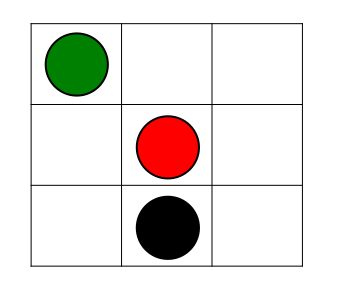
\includegraphics[width= 0.45\textwidth]{./images/nachbarn.png}
\caption{Ein 3x3 Raster mit Zellen in drei verschiedenen Zuständen}
\label{fig:Raster}
\end{figure}

\subsection*{Zelluläre Automaten}
Die vorliegende Implementierung basiert auf zellulären Automaten. Das heißt das jede Zelle erst einmal für sich unabhängig von anderen Zellen existiert.Eine Zelle ist im Kontext dieser Arbeit ein Mensch oder ein Tier. Dabei kann sich die Zelle in jeder Phase der Simulation nur in genau einem der folgenden Zustände befinden:
\begin{enumerate}
\item{\emph{Anfällig}\\
Eine anfällige Zelle kann nur von infizierten Zellen in ihrem direkten Umfeld welches durch eine Moore-Nachbarschaft \cite{Weisstein:2014} des Radius 1 charakterisiert wird angesteckt werden. Daraus folgt, dass eine Zelle auf dem rechteckigen Raster nur von den Zellen links über ihr, direkt über ihr, rechts über ihr, links und rechts neben ihr und links neben ihr, links unter ihr, direkt unter ihr und rechts unter ihr angesteckt werden kann.Dies sind im inneren des Spielfeldes maximal acht Zellen wie man am Beispiel der roten Zelle in Abbildung \ref{fig:Raster} gut sehen kann.\\
Des Weiteren wird auch betrachtet ob die Krankheit auch von jeder Zelle auf jede übertragbar ist oder ob zum Beispiel nur eine Übertragung von Mensch auf Tier aber nicht von Mensch auf Mensch möglich ist.\\
Angenommen die rote Zelle in Abbildung \ref{fig:Raster} ist ein infizierter Mensch und  die grüne Zelle ein gesundes Tier und die simulierte Krankheit lässt sich nicht von Mensch auf Tier übertragen. Demzufolge ist die grüne Zelle zu diesem Zeitpunkt vollkommen sicher, da sich in ihrer Nachbarschaft keine für sie potentiell gefährlichen Zellen befinden. 
}
\item{\emph{Infiziert}\\
Eine infizierte Zelle kann an ihrer Krankheit sterben, heilen und damit in den ersten Zustand übergehen, eine Resistenz bilden und damit in den dritten Zustand übergehen oder sie bleibt weiterhin infiziert.\\
All dies geschieht unter Berücksichtigung der für die simulierte Krankheit eingegebenen Werte.\\
Des Weiteren kann sie natürlich alle gesunden Zellen in ihrem Umfeld infizieren, auch dies geschieht unter Berücksichtigung der Werte die für die aktuelle Krankheit gelten.
}
\item{\emph{Resistent}\\
Da resistente Zellen nicht mehr in den Infiziert Zustand übergehen können und das Programm keine natürlichen Tode vorsieht, sind diese Zellen im Kontext des Programms unsterblich.\\
Sie werden jedoch trotzdem betrachtet, da sie im Kontext der Simulation interessant sind. So könnte man beispielsweise betrachten wie sich eine Krankheit verbreitet wenn bereits fast alle Zellen immun sind und es nur sehr wenige infizierte und anfällige Zellen gibt. Denkbar ist in diesem Szenario, dass die resistenten Zellen die infizierten Zellen weitestgehend abschirmen und so eine weitere Verbreitung verhindern. 
}

\item{\emph{Tot}\\
Eine Zelle in diesem Zustand, ist für die weitere Simulation nicht relevant. Naheliegenderweise kann sie sich nicht mehr eigenständig bewegen und auch kann sie keine anderen Zellen mehr infizieren. Es mag zwar durchaus Krankheiten geben welche auch nach dem Tot des Wirtes infektiös, an dieser Stelle wird in der Simulation davon ausgegangen dass die Zelle sich in einem intaktem Umfeld befindet in dem Tote entweder isoliert werden, dass sie keinen Kontakt mehr zu lebendigen Individuen haben. 
}
\end{enumerate}

\subsection*{Bewegung}
Zellen die sich in einem der ersten drei Zustände befinden können sich bewegen. Dabei wird in dieser Simulation davon ausgegangen dass die Zellen sich in einem geschlossenem Umfeld befinden. Es können also keine Zellen das Simulationsgebiert verlassen oder neu betreten.\\
Des Weiteren handelt es sich um eine zweidimensionale Simulation in der es nicht möglich ist dass sich mehrere Zellen auf einem Feld über- oder untereinander befinden.\\
Im allgemeinen Fall bewegen sich die Zellen dem Simple Isotropic  Random Walk Model \cite{Codling:2008} entsprechend, dies bedeutet dass sich eine Zelle zufällig in irgendeine Richtung bewegt unabhängig davon wohin sie sich zuvor bewegt hat. Dabei wird davon ausgegangen dass die Zellen grundsätzlich einen Drang zur Bewegung haben.\\
Sollte sich eine Zelle jedoch entscheiden sich in ein Feld zu bewegen indem schon eine andere Zelle ist, ist diese Bewegung nicht möglich und die Zelle muss sich neu entscheiden. Das Gleiche gilt für Zellen am Rand des Simulationsgebietes. Natürlich gibt es die Möglichkeit dass eine Zelle komplett \glqq umringt\grqq\; von anderen Zellen ist, in diesem Fall bleibt die Zelle zwangsweise an ihrer alten Position.\\
Veranschaulicht bedeutet dass das zum Beispiel die grüne Zelle in Abbildung \ref{fig:Raster} nur zwei Möglichkeiten hat sich zu bewegen. Nämlich eine Bewegung nach unten oder nach rechts. Da über und links neben ihr keine Felder mehr sind und auf der Diagonale kann sie sich auch nicht bewegen da dort die rote Zelle das einzig mögliche Feld blockiert.\\
%Quelle hier einbinden
\subsection*{Wirtsbeziehungen}
Die Simulation ist in der Lage einfache Wirtsbeziehungen zu simulieren, dadurch dass es zwei Arten von Zellen gibt (Menschen und Tiere), kann man krankheitsabhängig unterscheiden ob eine Krankheit jeweils von Mensch auf Mensch, von Mensch auf Tier, von Tier auf Mensch und von Tier auf Tier übertragbar ist, so kann schon eine beträchtliche Menge von Krankheiten simuliert werden.\\
Dies ermöglicht es zu simulieren was passiert wenn man versucht Krankheiten wie die Tollwut welche fast ausschließlich von Tieren auf den Mensch übertragen werden, versucht auszurotten indem man alle potentiellen Wirte immunisiert.

\subsection*{Bevölkerungsdichte}
Im Rahmen dieses Modell ist es möglich zu simulieren wie sich eine Krankheit bei verschiedener Bevölkerungsdichte verhält. So ist es möglich dass es auf einem gegebenem Raster $x\cdot y$ für die gilt $ x,y \in \mathbb{N}$ zwischen $1$ und $x\cdot y$ Zellen zu platzieren.\\
Dabei ist auch das Verhältnis von Menschen zu Tieren vollkommen beliebig wählbar. So lassen sich die Auswirkungen der Bevölkerungsdichte auf die Entwicklung simulieren.

\subsection*{Nicht deterministisch}
Ob eine Zelle in einen bestimmten Zustand übergeht hängt einerseits von ihrem eigenem Zustand und den Zuständen ihrer Nachbarn, andererseits von einer krankheitstypischen Wahrscheinlichkeit ab. Sollte eine Zelle infiziert sein und bei der simulierten Krankheit besteht die Wahrscheinlichkeit zu sterben bei 25\% so wird der Wert 0.25 mit einer zufälligen Zahl zwischen 0 und 1 verglichen. Sollte diese Zufallszahl größer sein als die Übergangswahrscheinlichkeit geht die Zelle in den entsprechenden Zustand über.\\
Das bedeutet das selbst wenn man die Simulation mit exakt den selben Parametern mehrmals durchführt man unterschiedliche Ergebnisse erzielen kann. Das Modell ist also nicht deterministisch.


%\begin{enumerate}
%\item{Bewegung}
%\item{\emph{Wirtsbeziehungen}
%
%
%
%}
%\item{\emph{Bevölkerungsdichte wird berücksichtigt}
%
%
%}
%\item{nicht deterministisch}
%\end{enumerate}
